% #######################################
% ########### FILL THESE IN #############
% #######################################
\def\mytitle{Cipher Website Report}
\def\mykeywords{Cipher Website Report}
\def\myauthor{Christopher Jones}
\def\contact{40274924@napier.live.ac.uk}
\def\mymodule{Web Tech(SET08101)}
% #######################################
% #### YOU DON'T NEED TO TOUCH BELOW ####
% #######################################
\documentclass[10pt, a4paper]{article}
\usepackage[a4paper,outer=1.5cm,inner=1.5cm,top=1.75cm,bottom=1.5cm]{geometry}
\twocolumn
\usepackage{graphicx}
\graphicspath{{./images/}}
%colour our links, remove weird boxes
\usepackage[colorlinks,linkcolor={black},citecolor={blue!80!black},urlcolor={blue!80!black}]{hyperref}
%Stop indentation on new paragraphs
\usepackage[parfill]{parskip}
%% Arial-like font
\usepackage{lmodern}
\renewcommand*\familydefault{\sfdefault}
%Napier logo top right
\usepackage{watermark}
%Lorem Ipusm dolor please don't leave any in you final report ;)
\usepackage{lipsum}
\usepackage{xcolor}
\usepackage{listings}
%give us the Capital H that we all know and love
\usepackage{float}
%tone down the line spacing after section titles
\usepackage{titlesec}
%Cool maths printing
\usepackage{amsmath}
%PseudoCode
\usepackage{algorithm2e}

\titlespacing{\subsection}{0pt}{\parskip}{-3pt}
\titlespacing{\subsubsection}{0pt}{\parskip}{-\parskip}
\titlespacing{\paragraph}{0pt}{\parskip}{\parskip}
\newcommand{\figuremacro}[5]{
    \begin{figure}[#1]
        \centering
        \includegraphics[width=#5\columnwidth]{#2}
        \caption[#3]{\textbf{#3}#4}
        \label{fig:#2}
    \end{figure}
}

\lstset{
	escapeinside={/*@}{@*/}, language=C++,
	basicstyle=\fontsize{8.5}{12}\selectfont,
	numbers=left,numbersep=2pt,xleftmargin=2pt,frame=tb,
    columns=fullflexible,showstringspaces=false,tabsize=4,
    keepspaces=true,showtabs=false,showspaces=false,
    backgroundcolor=\color{white}, morekeywords={inline,public,
    class,private,protected,struct},captionpos=t,lineskip=-0.4em,
	aboveskip=10pt, extendedchars=true, breaklines=true,
	prebreak = \raisebox{0ex}[0ex][0ex]{\ensuremath{\hookleftarrow}},
	keywordstyle=\color[rgb]{0,0,1},
	commentstyle=\color[rgb]{0.133,0.545,0.133},
	stringstyle=\color[rgb]{0.627,0.126,0.941}
}

\thiswatermark{\centering \put(336.5,-38.0){
\includegraphics[scale=0.8]{logo}} }
\title{\mytitle}
\author{\myauthor\hspace{1em}\\\contact\\Edinburgh Napier University\hspace{0.5em}-\hspace{0.5em}\mymodule}
\date{}
\hypersetup{pdfauthor=\myauthor,pdftitle=\mytitle,pdfkeywords=\mykeywords}
\sloppy
% #######################################
% ########### START FROM HERE ###########
% #######################################
\begin{document}
	\maketitle

	
\section {Introduction}
The main aim of this website was to show of 3 different ciphers in a simple and easy to use web page. The first cipher I chose to implement was the Caesar cipher as it seemed to be a cipher that was more complex than others i had looked at and felt that my website needed at least one strong cipher. The second cipher I chose was Atbash because it was relativity simple yet did require a bit of thinking to do once I had read into it a bit. The final cipher i chose to implement was the binary cipher which was the easiest of all the ciphers but still offers quite a good purpose for scrambling messages. To complete these 3 ciphers especially Caesar I used \href{https://en.wikipedia.org/wiki/Caesar_cipher}{Caesar Cipher Wiki} to understand what had to be done as it has a couple of great examples that are easy to follow and implement yourself.

\section {Software Design}
I planned each of the cipher web pages to be based on the same design so that the user can easily navigate and use each one as once the user can use one then they can effectively use the others. I mentioned this before but I wanted my website to be very simplistic and easy to use and understand as I didn't want to confuse the user.
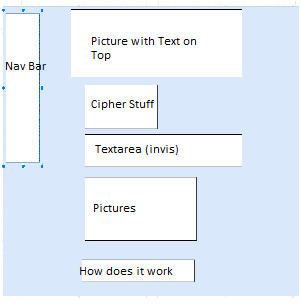
\includegraphics{Capture.PNG}
As you can see from my plan above I had a set structure that i wanted to keep to and this how each cipher Web page is laid out. Where it is says "pictures" on the picture I had a pretty good idea of what I wanted to do. Instead of just having still images i knew HTML and CSS were able to move pictures inside a set container on the screen using the marquee tag. I had learned this at school and knew if i found the right picture for each the ciphers I could make a cool effect. For the "how does it work" I wanted to make it like a Reddit page where there will a TL;DR because every time I read Reddit and see a huge long post that I really am to lazy to read then I use the TL;DR that the original poster has provided. So my plan was to implement one into my website so that other lazy people can have a simplified version of how it works. The homepage was a different story as I didn't create a physical plan for that I sort of had a plan inside my head for it. I wanted to make it semi funny to keep peoples attention as a user attention can be lost on a website of they don't see an interesting title or picture. To do this I want to put meme on the front which should work quite well in keeping people on the web page even though it will have no relevance to the ciphers. To navigate from the homepage I knew i didn't want to have a navigation bar but instead wanted hyper links on the 3 pictures that correspond to each of the ciphers and the design page. My main plan for the homepage was to keep it pretty basic and didn't want to try and do anything that I knew would take a lot of time to implement as I am great at planning things but not good at actually making that plan look good (designing).
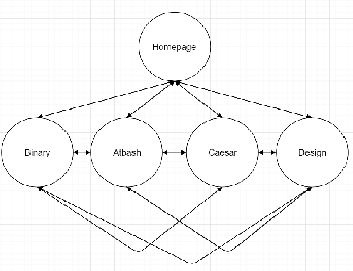
\includegraphics{nav.png}
As can be seen from the picture my plan for the navigation was to have nothing linear and how the user to get to any Web page no matter where they were on the website because linear websites are just annoying to get around on. Also the website doesn't have a lot of web pages so that makes it even easier to implement the navigation as a spiders web rather than having each web page lead onto the next or whatever.


\section{Implementation}
My website was solely implemented using HTML and CSS for the design of each Web page and JavaScript was used for the scripts which actually contain the functions for the ciphers. I think the homepage was very easy to implement. The hardest thing was the title which required to have text on top of an image which was done first by creating a container in CSS and telling CSS where the enter of the page actually is as that is where you want the banner to be.

\begin{lstlisting}
.container {
    position: relative;
    text-align: center;
    color: white;
}
.centered {
    position: absolute;
    top: 50%;
    left: 50%;
    transform: translate(-50%, -50%);
}

\end{lstlisting}
Once the container has been set up then it was possible to tell the CSS what image is to be put in the container and then call the class that tells the HTML to centre of the Web Page. Finally once the picture is there we can write on top of it which can be seen below. 
\begin{lstlisting}
<div class = "container">
		<img src="binary.jpg" height="200" width="1080" alt = ""/>
		<div class="centered"><h1><font color="black"><div class = "body"> Welcome to the Ciphers Web page:<br />  Created by Chris Jones </font></h1></div>
		</div>
\end{lstlisting}
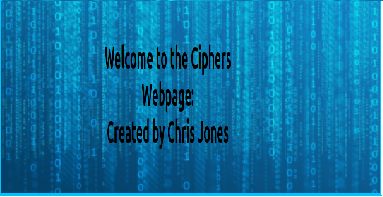
\includegraphics{images/banner.png}
The image above is the final outcome of the CSS and HTML and works quite nice as a banner.
I think the hardest cipher to implement on this website was by far the Caesar cipher mainly because i kept spelling it wrong and was wondering why my function wouldn't run but because it was the most complex out of all 3 of them.
\begin{lstlisting}
function caeserEncrypt(){

	var word = document.getElementById('word').value;
	var shift = document.getElementById('shift').value;

	var output = '';

	shift = parseInt(shift);

	for (var i = 0; i < word.length; i++){

		var character = word[i];

		if(character.match(/[a-z]/i)){

			var uniCode = character.charCodeAt(0);

			//uppercase
			if ((uniCode >= 65) && (uniCode <= 90)){
				uniCode += shift;
				if(uniCode > 90){
					uniCode -= 26;
				}
			} //lowercase
			else if((uniCode >= 97) && (uniCode <= 122)){
				uniCode += shift;
				if(uniCode > 122){
					uniCode -= 26;
				}
			}
    character = String.fromCharCode(uniCode);

		}

		output += character;
	}
\end{lstlisting}
The JavaScript above shows how the Caesar encrypt is implemented. Once you have your head around how the Unicode works then it wasn't too bad but trying to find where upper and lower case letters start was pretty annoying. The basic concept of it though is it loops around each character and finds its Unicode equivalent. Then that can be checked to see if its upper or lowercase and then the shift is added which the user enters in. If the Unicode goes outside the upper or lowercase range then minus the alphabet to get back to the beginning. Finally the characters are put back into there string equivalent and adds to the output.
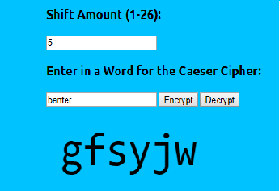
\includegraphics{images/Caesar.PNG}
The output of the Caesar cipher can be see above with a shift of 5 and the word being banter (bad image the template makes it hard to scale pictures properly). The scrambled word can be seen below and only decrypted with the same shift put in. This was roughly the same implementation for all of the ciphers as i have already mentioned the web pages were designed so once you learn one then you can use the others. The only difference between them is what cipher they use and the pictures but in all other regards they are effectively the same template. 


\section{Critical Evaluation}
My plan was there and I had really thought about how I wanted my website to look however I think the implementation was sloppy as the home page in itself not the greatest and needs some TLC to fix and flatten out some issues. However, in saying that I do think throughout its problems the homepage does do its job of allowing the user to navigate around the website even though its not the most elegant way of doing it. I think i did miss out on a lot of extra features that the homepage could of had for instance links to the actual cipher wikis to help user understand more about them than I could tell them. I also think my design document may be a tad full on for the user to understand as I'm not the best at explaining things and probably over complicate things are normally relatively easy. It is also missing out on some design issues that i would have like to implement like snippets are code appearing on scream but due to time constraints it wasn't really viable to try and to extra stuff that could impede on the overall project of the website. One other thing that i will probably improve for next time is the colour scheme which i personally quite liked the black on the blue is a bit of a dull colour scheme and might make users leave the website when they see it which is potentially a very big problem. One thing I would have loved to do if i had more time was to try and implement the play fair cipher which i did try and is in the git hub repository but serves no purpose. The Caesar cipher is sort of the mid range of hard to implement but play fair would have really made my website stand out however trying to get the square using a 2D array proved a bit too difficult to it was quickly abandoned after several hours of getting annoyed. I think the last thing that i may improve for next time is not leaving so much white space(blue space in my case) on the some of the pages which i think i probably could have fixed by messing around with the CSS a bit but never got around to do doing that unfortunately.
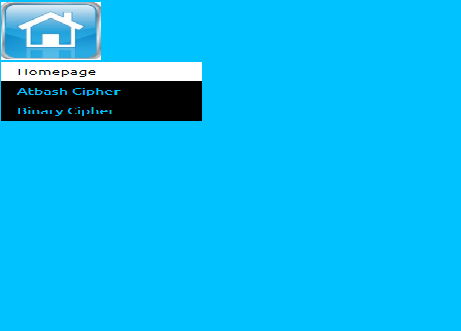
\includegraphics{images/WhiteSpace.png}
As can be seen with the image above even though it is shrunk a bit there is a ton of just nothing before any text off to the right which i think really needs to be fixed as its just an eye sore to look at.

\section{Personal Evaluation}
I learned a lot from this coursework especially about JavaScript which i did a bit at school but using it for Unity rather than anything web based which was different. One of the biggest and most annoying challenges i faced was HTML/CSS for its dreadful scaling for different resolutions. Going from 3840 x 2160 (4K) to 1920 x 1080 (1080p) and my Macs weird resolution of 1440 x 900 because Apple. It causes a lot of problems because i mainly did the JavaScript at 1080p but put the website on the 4K monitor it looked amazing at 4K everything nice and aligned but as soon as you move it to 1080p, it just breaks with images getting pushed down a line because there isn't enough space on the monitor. This was most prevalent on the homepage with my picture navigation which I had to redesign everything for 1080p monitors as that is the standard these days. Another problem was the fact that using the <form> tag would break my textarea for some reason. It basically refreshed the page and removed the decrypted word and it took me some time to find what the cause of the problem actually was because it wasn't that obvious until i began messing around with the tags and seeing which one caused the problem. I think the last problem that had a pretty big impact was the fact that used to have a black background with a really dark blue text which looked again alright on some monitors that had a good colour range but bad on ones that didn't as it was pretty unreadable. As again i had worked at 4K which gets a pretty good score on the adobe colour wheel but as soon as i moved it to my 1080p monitor you couldn't see what any of it said. I solved this by downloading a colour wheel package in Atom which allowed me to get RGB or HEX values for my website and hence how i got the baby blue. I'm going to say this now i am not good a design never have been so my website is a interesting blend of things some people think it doesn't look the greatest and i agree but its all about the perception of the user. Overall I'm pleased with how it actually turned out although things could be changed and tweaked, it wasn't as bad as the first iteration and only got better the more i worked on it :D 

\bibliographystyle{ieeetr}
\begin{thebibliography}{9}
\bibitem{Atbash}
Atbash PNG,
\\\texttt{https://aminoapps.com/c/cartoon/page/blog/gravity-falls}
\\\texttt{-how-to-learn-atbash-cipher/ER1I_PuxaqDYqpv75xa1zPgmaB}
\\\texttt{88lMb}.

\bibitem{binary}
Binary PNG,
\\\texttt{https://www.hdwallpapers.in/matrix_binary-wallpapers.html}

\bibitem{Caesar}
Caesar PNG,
\\\text{https://www.amazon.com/14th-Place-Trading-CCC03-Decoder}
\\\text{/dp/B004J43DWK}

\bibitem{Hello There Gif}
Hello There Gif,
\\\texttt{https://giphy.com/gifs/star-wars-the-phantom-menace}
\\\texttt{-hello-there-KOVlHmbBA09XO}

\bibitem{HomeButton}
Home Button JPG
\\\texttt{https://www.google.co.uk/search?q=homepage+button&}
\\\texttt{rlz=1C1CHBF_en-GBGB757GB757&source=lnms&tbm=isch&sa=X&ved=0ahUKEwjb_6iN7cPZAhXrCcAKHRxkArIQ_AUICigB&biw=2559&bih=1333#imgrc=PKGHl5C7eeZTaM}

\bibitem{Binary}
Binary Gif
\\\text{https://giphy.com/gifs/code-ko7twHhomhk8E}

\bibitem{Stack Overflow}
Stack Overflow for the textarea
\\\text{https://stackoverflow.com/}

\bibitem{Wiki}
Wiki for the ciphers
\\\text{https://en.wikipedia.org/wiki/Main_Page}
\end{thebibliography}		




		
\end{document}
